\documentclass[aspectratio=149, dvipsnames]{beamer}
% \documentclass[aspectratio=149, dvipsnames, handout]{beamer}
\usetheme{Inf}
\usepackage{xcolor}
\usepackage[T1]{fontenc}
\usepackage[utf8]{inputenc}

\usepackage{pifont}

\usepackage{venturis}

\setlength{\parskip}{.3em}
\usepackage{indentfirst}

\usepackage{amssymb}
\usepackage{amsmath}
\usepackage[ruled,vlined,linesnumbered]{algorithm2e}
\usepackage{mathtools}
\usepackage{booktabs}
\usepackage{graphicx}
\usepackage{xparse}
\usetikzlibrary{fit,shapes.misc, calc}

\usepackage{tikz}
\usetikzlibrary{positioning, arrows.meta, patterns, automata}
\tikzstyle{black_node}=[circle, draw, very thick, minimum height=8mm, minimum width=8mm]
\tikzstyle{black_rec_node}=[draw, very thick, minimum height=8mm, minimum width=8mm]

\usepackage{macros}

\title
[
    \textbf{Dead Ends in FOND}
]
{
    Dead Ends in FOND Planning: \\ {\small From Theory to Practical Contributions}
}

\author
[
    Marco Chitolina
]
{
    \centering \footnotesize\textcolor{darkgray}{} \\[-7pt]
}

\institute
{
    \small \textcolor{black}{Marco Antônio Chitolina} \\[-8pt]
}

\date
{
    Advisor: \textcolor{black}{Prof.~Dr. André Grahl Pereira} \\[-2pt]
    Co-advisor: \textcolor{black}{B. Sc. Frederico Messa}\\[-2pt]
    Federal University of Rio Grande do Sul
}

\AtBeginSection
{
    \setbeamercolor{footline}{fg=InfWhite}
    \begin{frame}[noframenumbering]
        \begin{huge}
            \begin{center}
                \insertsection
            \end{center}
        \end{huge}
    \end{frame}
    \setbeamercolor{footline}{fg=InfBlack}
} 

\begin{document}

\InfTitlePage
\setbeamercolor{footline}{fg=InfBlack}
\section{Introduction.}
\begin{frame}{Fully Observable Non-Deterministic (FOND) planning.}
    A framework for solving sequential decision problems with \textbf{uncertainty}.
\end{frame}
\begin{frame}{Motivation.}\pause
\textbf{Problem:} \pause PR2 easily solves all instances in the benchmarks used by the FOND community.\pause

\textbf{Our approach:} \pause study which factors are more relevant for a FOND task's difficulty. \pause
Use this knowledge to build a new benchmark.
\end{frame}

\begin{frame}{Presentation Flow.}\pause
    \begin{itemize}
        \item FOND task. \pause
        \item Dead ends in FOND planning. \pause
        \item Finding all dead ends in a FOND task. \pause
        \item What makes a FOND planning task difficult to solve? \pause
        \item New benchmark. \pause
        \item Evaluating new benchmark. \pause
        \item Discussion and future work.
    \end{itemize}
\end{frame}

% \begin{frame}{Thesis Statement}
%     \begin{quote}
%         \textit{``\textbf{Explicit policy-space heuristic search} should be an \textbf{effective way} of solving \textbf{FOND planning tasks}.''}
%     \end{quote}
% \end{frame}

\section{Background.}
% \begin{frame}{State-space search with non-determinism.}
%     \input{graphs/graph1}
% \end{frame}
\begin{frame}{FOND planning Task.} \pause
    \begin{columns}
        \begin{column}{.38\textwidth}
            \begin{itemize}
                \visible<2->{\item Set of states $\states$}
                \visible<4->{\item Initial state $s_0$}
                \visible<6->{\item Set of goal states $\states^*$}
                \visible<8->{\item Set of actions $\actions$}
            \end{itemize} 
        \end{column}%
        \hfill%
        \begin{column}{.58\textwidth}
            \begin{figure}
                \centering
                \scalebox{0.7}
                {
                    \only<2-4>{\visible<3-4>{\input{graphs/graph-1-states}}}%
                    \only<5-6>{\centering
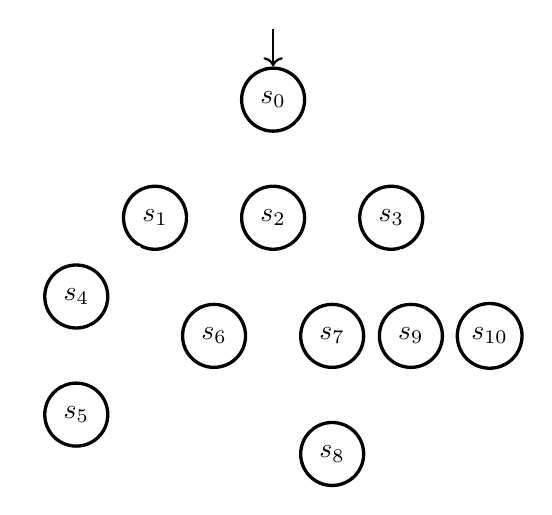
\begin{tikzpicture}
    \node[black_node] at ( 0.0,  0.0) (s0) {$s_0$};
    \node[black_node] at ( -1.5,  -1.5) (s1) {$s_1$};   
    \node[black_node] at ( 0,  -1.5) (s2) {$s_2$};  
    \node[black_node] at ( 1.5,  -1.5) (s3) {$s_3$}; 
    \node[black_node] at ( -2.5,  -2.5) (s4) {$s_4$};   
    \node[black_node] at ( -2.5,  -4.0) (s5) {$s_5$};   
    \node[black_node] at ( -.75,  -3) (s6) {$s_6$};  
    \node[black_node] at ( .75,  -3) (s7) {$s_7$};  
    \node[black_node] at ( .75,  -4.5) (s8) {$s_8$};   
    \node[black_node] at (1.75,  -3) (s9) {$s_9$};
    \node[black_node] at (2.75,  -3) (s10) {$s_{10}$};   
    
    \draw[->, thick] ( 0.0, 0.9) -- (s0) ;
    \draw[->, thick, color=white] (s0) to [bend left=25] (s1) ;     \draw[->, thick, color=white] (s1) to [bend left=25] (s0) ;
    \draw[->, thick, color=white] (s0) -- (s2);
    \draw[->, thick, color=white] (s0) -- (s3) ;
    \draw[->, thick, color=white] (s1.240) -- (s4) ;
    \draw[->, thick, color=white] (s1.240) -- (s6) ;
    \draw[->, thick, color=white] (s1.0) -- (s2) ;
    \draw[->, thick, color=white] (s4)  to [bend left=25] (s5) ;
    \draw[->, thick, color=white] (s5)  to [bend left=25] (s4) ;

    \draw[->, thick, color=white] (s2) -- (s7) ;
    \draw[->, thick, color=white] (s7) -- (s8) ;
    \draw[->, thick, color=white] (s8.130) -- (s6) ;
    \draw[->, thick, color=white] (s8.130)  to [bend left=25] (s2) ;
    
    \draw[->, thick, color=white] (s3.285) -- (s9) ;
    \draw[->, thick, color=white] (s3.285) -- (s10) ;

    \node[] at (0.55, -0.25) () {};
    \node[] at (-0.4, -0.55) () {};
    \node[] at (.20, -0.60) () {};
    \node[] at (-1.3, -2.1) () {};
    \node[] at (-1., -1.75) () {};
    \node[] at (-1.5, -.9) () {};
    \node[] at (.45, -1.90) () {};
    \node[] at (1.95, -1.90) () {};
    \node[] at (-2.1, -2.9) () {};
    \node[] at (-3., -3.50) () {};
    \node[] at (.95, -3.55) () {};
    \node[] at (0.2, -4.2) () {};
    \end{tikzpicture}}%
                    \only<7-8>{\input{graphs/graph-1-goal}}%
                    \only<9->{\input{graphs/graph-1}}%
                }
            \end{figure}
        \end{column}%
    \end{columns}%
\end{frame}

\begin{frame}{Policy.}\pause
 \begin{columns}
        \begin{column}{.5\textwidth}
            \begin{itemize}
                \visible<3->{\item\textbf{Policy / Plan:} describes what actions to apply in what states. }
                \visible<7->{\item \textbf{Solution:} policy that, when followed, ensures one parting from the initial state will eventually reach a goal.}
            \end{itemize} 
        \end{column}%
        \hfill%
        \begin{column}{.5\textwidth}
            \begin{figure}
                \centering
                \scalebox{0.8}
                {
                    %%%%%%%%%%%%%%%%%%%%
                    %% first policy 
                    %%%%%%%%%%%%%%%%%%%%
                    \only<-3>{\input{graphs/graph-1}}%
                    \only<4>{\input{graphs/graph-1-pol-2-1}}%
                    \only<5>{\input{graphs/graph-1-pol-2-2}}%
                    \only<6-7>{\input{graphs/graph-1-pol-2-3}}%
                    \only<8>{\input{graphs/graph-1-pol-2-4}}%

                    % % %%%%%%%%%%%%%%%%%%%%
                    % % %% second policy 
                    % % %%%%%%%%%%%%%%%%%%%%
                    \only<9>{\input{graphs/graph-1}}%
                    \only<10>{\input{graphs/graph-1-pol-1-8}}%
                    % \only<9>{\input{graphs/graph-1}}%
                    % \only<10>{\input{graphs/graph-1-pol-1-1}}%
                    % \only<11>{\input{graphs/graph-1-pol-1-2}}%
                    % \only<12>{\input{graphs/graph-1-pol-1-3}}%
                    % \only<13>{\input{graphs/graph-1-pol-1-4}}%
                    % \only<14>{\input{graphs/graph-1-pol-1-5}}%
                    % \only<15>{\input{graphs/graph-1-pol-1-6}}%
                    % \only<16>{\input{graphs/graph-1-pol-1-7}}%

                    % % %%%%%%%%%%%%%%%%%%%%
                    % % %% third policy 
                    % % %%%%%%%%%%%%%%%%%%%%
                    % \only<17>{\input{graphs/graph-1}}%
                    % \only<18>{\input{graphs/graph-1-pol-3-1}}%
                    % \only<19>{\input{graphs/graph-1-pol-3-2}}%
                    % \only<20>{\input{graphs/graph-1-pol-3-3}}%
                    % \only<21>{\input{graphs/graph-1-pol-3-4}}%
                    % \only<22>{\input{graphs/graph-1-pol-3-5}}%
                    \only<11>{\input{graphs/graph-1}}%
                    \only<12>{\input{graphs/graph-1-pol-3-4}}%
                    \only<13>{\input{graphs/graph-1-pol-3-5}}%
                }
            \end{figure}
        \end{column}%
    \end{columns}
\end{frame}
\begin{frame}{Dead ends.}\pause
 \begin{columns}
        \begin{column}{.5\textwidth}
            \begin{itemize}
                \only<1-2>{\item[]{}}
                \only<3-9>{\item\textbf{Dead-end state:} no goal-reachability guarantee.}
                \only<4-9>{
                \begin{itemize}
                \only<4-9>{\item\textbf{Deterministic:} no chance at all.}
                \only<6-9>{\item\textbf{Fully non-deterministic:} rely on luck.}
                \end{itemize}}
                \only<9>{\item\textbf{Alive state:} goal-reachability guarantee.}
                \only<10->{\item\textbf{Bad state-action pair:} may produce dead end.}
                % \only<12-13>{\item\textbf{Tricky state-action pair:} may produce both dead-end and alive state.}
            \end{itemize} 
        \end{column}%
        \hfill%
        \begin{column}{.5\textwidth}
            \begin{figure}
                \centering
                \scalebox{0.8}
                {
                    \only<-4>{\input{graphs/graph-1}}%
                    %\only<4-5>{\input{graphs/graph-1-dead-ends}}%
                    \only<5-6>{\input{graphs/graph-1-dead-ends-dde}}%
                    %\only<7>{\input{graphs/graph-1-dead-ends}}%
                    \only<7>{\input{graphs/graph-1-dead-ends-fndde}}%
                    \only<8>{\input{graphs/graph-1-dead-ends-fndde-trans}}%
                    \only<9-10>{\input{graphs/graph-1-dead-ends-fndde}}%
                    %\only<9-10>{\input{graphs/graph-1-dead-ends}}%
                    \only<11->{\input{graphs/graph-1-dead-ends-bsap}}%
                    % \only<13->{\input{graphs/graph-1-dead-ends-tsap}}%
                }
            \end{figure}
        \end{column}%
    \end{columns} 
\end{frame}
\section[Finding dead ends.]{Finding all dead ends in a FOND task.}
\begin{frame}{Procedure for finding all dead ends.} \pause
    Brute-Force Dead-End Detector (BFDED).\pause
    \begin{columns}
        \begin{column}{.38\textwidth}
            \begin{itemize}
                \only<-3>{\item[]{}}
                \only<4->{\item \textbf{Backward search} from each goal state.}
                \only<12->{\item Non-visited \textbf{states} are \textbf{deterministic} dead-ends.}
                \only<14->{\item \textbf{Actions} that generate them are \textbf{bad}.}
                \only<16>{\item Repeats.}
            \end{itemize} 
        \end{column}%
        \hfill%
        \begin{column}{.58\textwidth}
            \begin{figure}
                \centering
                \scalebox{0.7}
                {
                    \only<-4>{\input{graphs/graph-1}}%
                    \only<5>{\input{graphs/graph-1-bfded-1-1}}%
                    \only<6>{\input{graphs/graph-1-bfded-1-2-1}}%
                    \only<7>{\input{graphs/graph-1-bfded-1-2-2}}%
                    \only<8>{\input{graphs/graph-1-bfded-1-2-3}}%
                    \only<9>{\input{graphs/graph-1-bfded-1-3-1}}%
                    \only<10>{\input{graphs/graph-1-bfded-1-3-2}}%
                    \only<11-12>{\input{graphs/graph-1-bfded-1-4}}%
                    \only<13-14>{\centering
\begin{tikzpicture}
    \node[black_node] at ( 0.0,  0.0) (s0) {$s_0$};
    \node[black_node] at ( -1.5,  -1.5) (s1) {$s_1$};   
    \node[black_node] at ( 0,  -1.5) (s2) {$s_2$};  
    \node[black_node] at ( 1.5,  -1.5) (s3) {$s_3$}; 
    \node[black_node, fill=ddeState] at ( -2.5,  -2.5) (s4) {$s_4$};   
    \node[black_node, fill=ddeState] at ( -2.5,  -4.0) (s5) {$s_5$};   
    \node[black_node, accepting] at ( -.75,  -3) (s6) {$s_6$};  
    \node[black_node] at ( .75,  -3) (s7) {$s_7$};  
    \node[black_node] at ( .75,  -4.5) (s8) {$s_8$};   
    \node[black_node, accepting] at (1.75,  -3) (s9) {$s_9$};
    \node[black_node, fill=ddeState] at (2.75,  -3) (s10) {$s_{10}$};   
    
    \draw[->, thick] ( 0.0, 0.9) -- (s0) ;
    \draw[->, thick] (s0) to [bend left=25] (s1) ;     \draw[->, thick] (s1) to [bend left=25] (s0) ;
    \draw[->, thick] (s0) -- (s2);
    \draw[->, thick] (s0) -- (s3) ;

    \draw[->, thick] (s1.240) -- (s4) ;
    \draw[->, thick] (s1.240) -- (s6) ;
    \draw[->, thick] (s1.0) -- (s2) ;
    \draw[->, thick] (s4)  to [bend left=25] (s5) ;
    \draw[->, thick] (s5)  to [bend left=25] (s4) ;

    \draw[->, thick] (s2) -- (s7) ;
    \draw[->, thick] (s7) -- (s8) ;
    \draw[->, thick] (s8.130) -- (s6) ;
    \draw[->, thick] (s8.130)  to [bend left=25] (s2) ;
    
    \draw[->, thick] (s3.285) -- (s9) ;
    \draw[->, thick] (s3.285) -- (s10) ;
    
    \node[] at (0.55, -0.25) () {$e$};     \node[] at (-0.4, -0.55) () {$w$};     \node[] at (.20, -0.60) () {$s$};     \node[] at (-1.3, -2.1) () {$s$};     \node[] at (-1., -1.75) () {$e$};     \node[] at (-1.5, -.9) () {$n$};     \node[] at (.45, -1.90) () {$s$};     \node[] at (1.95, -1.90) () {$s$};     \node[] at (-2.1, -2.9) () {$s$};     \node[] at (-3., -3.50) () {$n$};     \node[] at (.95, -3.55) () {$s$};     \node[] at (0.2, -4.2) () {$n$};     \myCurveA     \myCurveB     \myCurveC \end{tikzpicture}}%
                    \only<15->{\input{graphs/graph-1-bfded-1-6}}%
            }
            \end{figure}
        \end{column}%
    \end{columns} 
\end{frame}
\addtocounter{framenumber}{-1}
\begin{frame}{Procedure for finding all dead ends.} 
    Brute-Force Dead-End Detector (BFDED).
    \begin{columns}
        \begin{column}{.38\textwidth}
            \begin{itemize}
                \only<1>{\item[]{}}
                \only<2->{\item \textbf{Backward search} from each goal state.}
                \only<9->{\item Non-visited \textbf{states} are \textbf{fully non-deterministic} dead-ends.}
                \only<11->{\item \textbf{Actions} that generate them are \textbf{bad}.}
                \only<13>{\item Repeats.}
            \end{itemize} 
        \end{column}%
        \hfill%
        \begin{column}{.58\textwidth}
            \begin{figure}
                \centering
                \scalebox{0.7}
                {
                    %%%%%%%%%%%%%%%%%%%%%
                    %% second iteration
                    %%%%%%%%%%%%%%%%%%%%%
                    \only<-2>{\input{graphs/graph-1-bfded-1-6}}%
                    \only<3>{\input{graphs/graph-1-bfded-2-1}}%
                    \only<4>{\input{graphs/graph-1-bfded-2-2}}%
                    \only<5>{\input{graphs/graph-1-bfded-2-3}}%
                    \only<6>{\input{graphs/graph-1-bfded-2-4}}%
                    \only<7>{\input{graphs/graph-1-bfded-2-5}}%
                    \only<8-9>{\input{graphs/graph-1-bfded-2-6}}%
                    \only<10-11>{\input{graphs/graph-1-bfded-2-7}}%
                    \only<12->{\input{graphs/graph-1-bfded-2-8}}%
            }
            \end{figure}
        \end{column}%
    \end{columns} 
\end{frame}
\addtocounter{framenumber}{-1}
\begin{frame}{Procedure for finding all dead ends.} 
    Brute-Force Dead-End Detector (BFDED).
    \begin{columns}
        \begin{column}{.38\textwidth}
            \begin{itemize}
                \only<-1>{\item[]{}}
                \only<2->{\item \textbf{Backward search} from each goal state.}
                \only<9->{\item No new dead end were found.}
                \only<11->{\item Procedure ends.}
                \only<12>{\item This process repeats at most $|\sets|$ times.}
            \end{itemize} 
        \end{column}%
        \hfill%
        \begin{column}{.58\textwidth}
            \begin{figure}
                \centering
                \scalebox{0.7}
                {
                    %%%%%%%%%%%%%%%%%%%%%
                    %% third iteration
                    %%%%%%%%%%%%%%%%%%%%%
                    \only<-2>{\input{graphs/graph-1-bfded-2-8}}%
                    \only<3>{\input{graphs/graph-1-bfded-3-1}}%
                    \only<4>{\input{graphs/graph-1-bfded-3-2}}%
                    \only<5>{\input{graphs/graph-1-bfded-3-3}}%
                    \only<6>{\input{graphs/graph-1-bfded-3-4}}%
                    \only<7>{\input{graphs/graph-1-bfded-3-5}}%
                    \only<8-9>{\input{graphs/graph-1-bfded-3-6}}%
                    \only<10->{\input{graphs/graph-1-bfded-2-8}}%
            }
            \end{figure}
        \end{column}%
    \end{columns} 
\end{frame}
% \begin{frame}{We genuinely tried to reduce BFDED's complexity and failed to do so.}
    
% \end{frame}

\section[Theoretical study.]{What makes a FOND planning task difficult to solve?}

\begin{frame}{The most naive way to solve a FOND task.}\pause
    Greedy Policy Maker (GPM$_0$).\pause
    \begin{columns}
        \begin{column}{.5\textwidth}
            \begin{itemize}
                \visible<4->{\item Selects a state.}
                \visible<6->{\item Maps it to an arbitrary action.}
                \visible<8->{\item Repeat.}
            \end{itemize} 
        \end{column}%
        \hfill%
        \begin{column}{.5\textwidth}
            \begin{figure}
                \centering
                \scalebox{0.8}
                {
                    \only<-4>{\input{graphs/graph-1}}%
                    \only<5-6>{\input{graphs/graph-1-gpm-1-0}}%
                    \only<7-8>{\input{graphs/graph-1-gpm-1-1}}%
                    \only<9>{\input{graphs/graph-1-gpm-1-2}}%
                    \only<10>{\input{graphs/graph-1-gpm-1-3}}%
                    \only<11>{\input{graphs/graph-1-gpm-1-4}}%
                    \only<12>{\input{graphs/graph-1-gpm-1-5}}%
                    \only<13>{\input{graphs/graph-1-gpm-1-6}}%
                }
            \end{figure}
        \end{column}%
    \end{columns} 
\end{frame}
\begin{frame}{What happens when we select the wrong action?}\pause
    Greedy Policy Maker (GPM$_0$).\pause
    \begin{columns}
        \begin{column}{.5\textwidth}
            \begin{itemize}
                \visible<4->{\item Selects a state.}
                \visible<6->{\item Maps it to an arbitrary action.}
                \visible<8->{\item Repeat.}
            \end{itemize} 
        \end{column}%
        \hfill%
        \begin{column}{.5\textwidth}
            \begin{figure}
                \centering
                \scalebox{0.8}
                {
                    \only<-4>{\input{graphs/graph-1}}%
                    \only<5-6>{\input{graphs/graph-1-gpm-1-0}}%
                    \only<7-8>{\input{graphs/graph-1-gpm-1-1}}%
                    \only<9>{\input{graphs/graph-1-gpm-5-1}}%
                    
                }
            \end{figure}
        \end{column}%
    \end{columns} 
\end{frame}
\begin{frame}{Deterministic distance to the goal might help.}\pause
    Greedy Policy Maker (GPM$_1$).\pause
    \begin{columns}
        \begin{column}{.5\textwidth}
            \begin{itemize}
                \visible<4->{\item \textbf{Deterministic distance to the goal}: in the best case, how many steps one must take to reach a goal.}
                \visible<6->{\item Selects a state.}
                \visible<8->{\item Maps it to an action whose successor state is one step closer to the goal.}
                \visible<10->{\item Repeat.}
            \end{itemize} 
        \end{column}%
        \hfill%
        \begin{column}{.5\textwidth}
            \begin{figure}
                \centering
                \scalebox{0.8}
                {
                    \only<-4>{\input{graphs/graph-1}}%
                    \only<5-6>{\input{graphs/graph-1-gpm-3-1}}%
                    \only<7-8>{\input{graphs/graph-1-gpm-3-2}}%
                    \only<9-10>{\input{graphs/graph-1-gpm-3-3}}%
                    \only<11>{\input{graphs/graph-1-gpm-3-4}}%
                    \only<12>{\input{graphs/graph-1-gpm-3-5}}%
                    \only<13>{\input{graphs/graph-1-gpm-3-6}}%
                }
            \end{figure}
        \end{column}%
    \end{columns} 
\end{frame}
\begin{frame}{Updating it dead-end information.}\pause
    Greedy Policy Maker (GPM$_2$). \pause
    \begin{columns}
        \begin{column}{.5\textwidth}
            \begin{itemize}
                \visible<4->{\item \textbf{Do not} consider any \textbf{bad} state-action pair.}
                \visible<6->{\item \textbf{Updated deterministic distance to the goal}: in the best case, how many steps one must take to reach a goal.}
                \visible<8->{\item Selects a state.}
                \visible<10->{\item Maps it to an action whose successor state is one step closer to the goal.}
                \visible<11->{\item Repeat.}
            \end{itemize} 
        \end{column}%
        \hfill%
        \begin{column}{.5\textwidth}
            \begin{figure}
                \centering
                \scalebox{0.8}
                {
                    \only<-4>{\input{graphs/graph-1}}%
                    \only<5-6>{\input{graphs/graph-1-bfded-2-8}}%
                    \only<7-8>{\input{graphs/graph-1-gpm-4-1}}%
                    \only<9>{\input{graphs/graph-1-gpm-4-2}}%
                    \only<10-11>{\input{graphs/graph-1-gpm-4-3}}%
                    \only<12>{\input{graphs/graph-1-gpm-4-4}}%
                    \only<13>{\input{graphs/graph-1-gpm-4-5}}%
                    \only<14>{\input{graphs/graph-1-gpm-4-6}}%
                    \only<15>{\input{graphs/graph-1-gpm-4-7}}%
                }
            \end{figure}
        \end{column}%
    \end{columns} 
\end{frame}

\begin{frame}{Where the difficulty lies in.}\pause
    Costs $\mathcal{O}(|\sets|^{1 + \epsilon})$:\pause
    \begin{itemize}
        \item \textbf{Finding all deterministic} dead ends.\pause
        \item Building \textbf{deterministic distances}.\pause
        \item Greedily \textbf{building a policy}.\pause
    \end{itemize} 
    If $\sets$ is small, can we solve the task? \pause Not necessarily! \pause GPM$_2$ still requires fully non-deterministic dead ends, and we do not know how to compute them in $\mathcal{O}(|\sets|^{1 + \epsilon})$.\pause
    
    If a FOND task does not have state space $\sets$ prohibitively large, \pause it can \textbf{only} be difficult if it contains fully non-deterministic dead ends.
\end{frame}
\section{New benchmark.}
\begin{frame}{Classical Benchmark.}
\scalebox{0.8}{
\begin{tabular}{l|c|c}
Domain & Has dead ends? & Has fully non-deterministic dead ends? \\
\hline
Acrobatics & \experimentSuccessStyle & \experimentFailStyle \\
Beam-walk & \experimentFailStyle & \experimentFailStyle \\
Blocks-world original & \experimentFailStyle & \experimentFailStyle \\
Blocks-world advanced & \experimentFailStyle & \experimentFailStyle \\
Chain of rooms & \experimentFailStyle & \experimentFailStyle \\
Doors & \experimentSuccessStyle & \experimentSuccessStyle \\
Earth observation & \experimentFailStyle & \experimentFailStyle \\
Elevators & \experimentFailStyle & \experimentFailStyle \\
Faults & \experimentFailStyle & \experimentFailStyle \\
First responders & \experimentSuccessStyle & \experimentSuccessStyle \\
Islands & \experimentSuccessStyle & \experimentFailStyle \\
Miner & \experimentSuccessStyle & \experimentFailStyle \\
Tire-world spiky & \experimentSuccessStyle & \experimentSuccessStyle \\
Tire-world truck & \experimentSuccessStyle & \experimentSuccessStyle \\
Tire-world triangle & \experimentSuccessStyle & \experimentSuccessStyle \\
Zeno & \experimentFailStyle & \experimentFailStyle \\
\end{tabular}}
\end{frame}
\begin{frame}{Classical Benchmark is no longer challenging.}
    \begin{itemize}
        \visible<2->{\item PR2 \textbf{easily} solves each domain task.}
        \visible<4->{\item Two-thirds of the domains have designs that \textbf{do not reflect} the \textbf{true nature} of FOND. }
        \visible<5->{\item They can only become difficult due to scale.}
        \visible<6->{\item This limits testing algorithms on real-world scenarios.}
    \end{itemize}
    \bigskip
    \visible<3->{\textbf{Easily}: under 6 minutes with 8GB of memory.}
\end{frame}
\begin{frame}{New benchmark.}
    \begin{itemize}
        \visible<2->{\item Relying on scaling up the instances is \textbf{not} worth it.}
        \visible<3->{\item Fully non-deterministic as the core characteristic of the design of our benchmark.}
        \visible<4->{\item Five domains, each with four instances.}
        \item[]\begin{itemize}
            \visible<5->{\item Kitchen.}
            \visible<6->{\item Rescue.}
            \visible<7->{\item Slippery sokoban.}
            \visible<8->{\item Tire-world spiky 2.}
            \visible<9->{\item Travelling salesman.}
        \end{itemize}
    \end{itemize}
\end{frame}
\begin{frame}{Kitchen.}
    \scalebox{0.75}{\label{tab:domain_specifications_kitchen}
\begin{tabular}{|l|l|} 
\hline
\keystyle{Domain} & \namestyle{Kitchen}\\
\hline
\keystyle{Type} & \typestyle{recipe}\\
\keystyle{} & \typestyle{ingredient}\\
\keystyle{} & \typestyle{customer}\\
% \keystyle{} & \typestyle{number} : $\{$ \predicatestyle{1}, \predicatestyle{2}, \predicatestyle{3}, \predicatestyle{$\dots$} $\}$\\
\hline
% \keystyle{Predicate} & \predicatestyle{next } (\variablestyle{n1}, \variablestyle{ n2 } : \typestyle{ number})\\
% \keystyle{} & \predicatestyle{finished } (\variablestyle{isl } : \typestyle{ number})\\
\keystyle{Constant Predicate} & \predicatestyle{on-recipe } (\variablestyle{ r } : \typestyle{recipe}) : \textbf{set}$\langle$\textbf{pair}$\langle$\typestyle{ingredient}, \typestyle{number}$\rangle$$\rangle$\\
\hline
\keystyle{Variable Predicate} & \predicatestyle{on-island } (\variablestyle{i } : \typestyle{ ingredient}) : \typestyle{ number}\\
% \keystyle{} & \predicatestyle{on-chef-island } (\variablestyle{i } : \typestyle{ ingredient}; \variablestyle{ n } : \typestyle{ number}; \variablestyle{ isl } : \typestyle{ number})\\
% \keystyle{} & \predicatestyle{not-on-recipe } (\variablestyle{i } : \typestyle{ ingredient}; \variablestyle{ r } : \typestyle{ recipe})\\
\keystyle{} & \predicatestyle{on-stock } (\variablestyle{i } : \typestyle{ ingredient}) : \typestyle{ number}\\
\keystyle{} & \predicatestyle{prepared } (\variablestyle{r } : \typestyle{ recipe}) : \typestyle{bool}\\
\keystyle{} & \predicatestyle{satisfied } (\variablestyle{c } : \typestyle{ customer}) : \typestyle{bool}\\
\keystyle{} & \predicatestyle{desired-recipes} (\variablestyle{c } : \typestyle{ customer}) : \textbf{set}$\langle$\typestyle{recipe}$\rangle$\\
% \keystyle{} & \predicatestyle{num-recipes-to-refuse } (\variablestyle{c } : \typestyle{ customer}; \variablestyle{ n } : \typestyle{ number})\\
% \keystyle{} & \predicatestyle{properly-added } (\variablestyle{i } : \typestyle{ ingredient}; \variablestyle{ r } : \typestyle{ recipe}; \variablestyle{ isl } : \typestyle{ number})\\
% \keystyle{} & \predicatestyle{can-use-chef-island } (\variablestyle{isl } : \typestyle{ number})\\
\hline
% \keystyle{Action} & \actionstyle{select-chef-island } (\variablestyle{isl } : \typestyle{ number})\\
\keystyle{Action} & \actionstyle{move-ingredient-to-island} (\variablestyle{i } : \typestyle{ ingredient}; \variablestyle{n } : \typestyle{ number})\\
\keystyle{} & \actionstyle{move-ingredient-to-stock} (\variablestyle{i } : \typestyle{ ingredient}; \variablestyle{n } : \typestyle{ number})\\
% \keystyle{} & \actionstyle{from-stock-to-chef-island } (\variablestyle{i } : \typestyle{ ingredient}; \variablestyle{ isl}, \variablestyle{ isl } : \typestyle{ number})\\
% \keystyle{} & \actionstyle{from-chef-island-to-stock } (\variablestyle{i } : \typestyle{ ingredient}; \variablestyle{ isl}, \variablestyle{ isl } : \typestyle{ number})\\
\keystyle{} & \actionstyle{select-recipe } (\variablestyle{r } : \typestyle{ recipe})\\
% \keystyle{} & \actionstyle{on-recipe-add-to-recipe } (\variablestyle{i } : \typestyle{ ingredient}; \variablestyle{ r } : \typestyle{ recipe}; \variablestyle{ isl}, \variablestyle{ n } : \typestyle{ number})\\
% \keystyle{} & \actionstyle{not-on-recipe-add-to-recipe } (\variablestyle{i } : \typestyle{ ingredient}; \variablestyle{ r } : \typestyle{ recipe}; \variablestyle{ isl } : \typestyle{ number})\\
\keystyle{} & \actionstyle{offer } (\variablestyle{c } : \typestyle{ customer}; \variablestyle{ r } : \typestyle{ recipe})\\
% \keystyle{} & \actionstyle{offer-not-refusable } (\variablestyle{c } : \typestyle{ customer}; \variablestyle{ r } : \typestyle{ recipe})\\
% \keystyle{} & \actionstyle{offer-refusable } (\variablestyle{c } : \typestyle{ customer}; \variablestyle{ r } : \typestyle{ recipe}; \variablestyle{ refused } : \typestyle{ number})\\
\hline
\end{tabular}
}
\end{frame}
\begin{frame}{Rescue.}
    \scalebox{0.6}{\begin{tabular}{|l|l|}
\hline
\keystyle{Domain} & \namestyle{Rescue}\\
\hline
\keystyle{Type} & \typestyle{location}\\
\keystyle{} & \typestyle{victim}\\
% \keystyle{} & \typestyle{fire-unit}\\
% \keystyle{} & \typestyle{medical-unit}\\
\keystyle{} & \typestyle{unit} \\
% \keystyle{} & \typestyle{number} : $\{$ \predicatestyle{1}, \predicatestyle{2}, \predicatestyle{3}, \predicatestyle{$\dots$} $\}$\\
\keystyle{} & \typestyle{status} : $\{$ \variablestyle{healthy}, \variablestyle{hurt}, \variablestyle{dying}, \variablestyle{deceased} $\}$\\
\hline
\keystyle{Constant Predicate} & \predicatestyle{water-supply-at } (\variablestyle{l } : \typestyle{ location}) : \typestyle{bool}\\
\keystyle{} & \predicatestyle{hospital-at } (\variablestyle{l } : \typestyle{ location}) : \typestyle{bool}\\
\keystyle{} & \predicatestyle{adjacent } (\variablestyle{l1}, \variablestyle{ l2 } : \typestyle{ location}) : \typestyle{bool}\\
\keystyle{} & \predicatestyle{critical-time } (\variablestyle{ l } : \typestyle{ location}) : \typestyle{ number}\\
\keystyle{} & \predicatestyle{is-medical-unit } (\variablestyle{u} : \typestyle{unit}) : \typestyle{bool}\\
\keystyle{} & \predicatestyle{is-fire-unit } (\variablestyle{u} : \typestyle{unit}) : \typestyle{bool}\\
\hline
\keystyle{Variable Predicate} & \predicatestyle{clock}() : \typestyle{number}\\
% \keystyle{Predicate} & \predicatestyle{clock } (\variablestyle{t } : \typestyle{ number})\\
% \keystyle{} & \predicatestyle{adjusted-clock }()\\
% \keystyle{} & \predicatestyle{is-greater-or-equal } (\variablestyle{n1}, \variablestyle{ n2 } : \typestyle{ number})\\
% \keystyle{} & \predicatestyle{inc } (\variablestyle{op}, \variablestyle{ res } : \typestyle{ number})\\
\keystyle{} & \predicatestyle{fire-at } (\variablestyle{l } : \typestyle{ location}) : \typestyle{bool} \\
\keystyle{} & \predicatestyle{victim-at} (\variablestyle{v} : \typestyle{ victim}) : \textbf{either} \typestyle{ location} \textbf{or} \typestyle{ unit}\\
% \keystyle{} & \predicatestyle{fire-unit-at } (\variablestyle{u } : \typestyle{ fire}; \variablestyle{ unit}, \variablestyle{ l } : \typestyle{ location})\\
% \keystyle{} & \predicatestyle{medical-unit-at } (\variablestyle{u } : \typestyle{ medical}; \variablestyle{ unit}, \variablestyle{ l } : \typestyle{ location})\\
\keystyle{} & \predicatestyle{unit-at} (\variablestyle{u} : \typestyle{unit}) : \typestyle{ location}\\
\keystyle{} & \predicatestyle{loaded} (\variablestyle{u} : \typestyle{unit}) : \textbf{either} \typestyle{bool} \textbf{or} \typestyle{victim}\\
% \keystyle{} & \predicatestyle{healthy } (\variablestyle{v } : \typestyle{ victim})\\
% \keystyle{} & \predicatestyle{hurt } (\variablestyle{v } : \typestyle{ victim})\\
% \keystyle{} & \predicatestyle{dying } (\variablestyle{v } : \typestyle{ victim})\\
% \keystyle{} & \predicatestyle{deceased } (\variablestyle{v } : \typestyle{ victim})\\
% \keystyle{} & \predicatestyle{spread-out } (\variablestyle{t } : \typestyle{ number}; \variablestyle{ l } : \typestyle{ location})\\
%  \keystyle{} & \predicatestyle{adjusted-status } (\variablestyle{t } : \typestyle{ number}; \variablestyle{ v } : \typestyle{ victim})\\
% \keystyle{} & \predicatestyle{need-to-adjust-clock }()\\
% \keystyle{} & \predicatestyle{have-water } (\variablestyle{u } : \typestyle{ fire})\\
% \keystyle{} & \predicatestyle{have-victim-in-unit } (\variablestyle{v } : \typestyle{ victim}; \variablestyle{ u } : \typestyle{ medical})\\
\keystyle{} & \predicatestyle{in-hospital } (\variablestyle{v } : \typestyle{ victim}) : \typestyle{bool}\\
\keystyle{} & \predicatestyle{is } (\variablestyle{v } : \typestyle{ victim}) : \typestyle{ status}\\
% \keystyle{} & \predicatestyle{predecessor-victim } (\variablestyle{v1}, \variablestyle{ v2 } : \typestyle{ victim})\\
% \keystyle{} & \predicatestyle{predecessor-location } (\variablestyle{l1}, \variablestyle{ l2 } : \typestyle{ location})\\
% \keystyle{} & \predicatestyle{all-locations-spread-out } (\variablestyle{t } : \typestyle{ number})\\
% \keystyle{} & \predicatestyle{all-victims-adjusted } (\variablestyle{t } : \typestyle{ number})\\
% \keystyle{} & \predicatestyle{first-victim } (\variablestyle{v } : \typestyle{ victim})\\
% \keystyle{} & \predicatestyle{first-location } (\variablestyle{l } : \typestyle{ location})\\
\hline
\keystyle{Action} & \actionstyle{drive} (\variablestyle{u} : \typestyle{unit}; \variablestyle{ from }, \variablestyle{ to } : \typestyle{ location})\\
% \keystyle{Action} & \actionstyle{drive-fire-unit } (\variablestyle{u } : \typestyle{ fire}; \variablestyle{ unit}, \variablestyle{ from } : \typestyle{ location}; \variablestyle{ to } : \typestyle{ location})\\
% \keystyle{} & \actionstyle{drive-medical-unit } (\variablestyle{u } : \typestyle{ medical}; \variablestyle{ unit}, \variablestyle{ from } : \typestyle{ location}; \variablestyle{ to } : \typestyle{ location})\\
\keystyle{} & \actionstyle{load-fire-unit} (\variablestyle{u} : \typestyle{unit})\\
\keystyle{} & \actionstyle{load-medical-unit} (\variablestyle{u} : \typestyle{unit}; \variablestyle{v} : \typestyle{victim})\\
% \keystyle{} & \actionstyle{load-fire-unit } (\variablestyle{u } : \typestyle{ fire}; \variablestyle{ unit}, \variablestyle{ l } : \typestyle{ location})\\
% \keystyle{} & \actionstyle{load-medical-unit } (\variablestyle{u } : \typestyle{ medical}; \variablestyle{ unit}, \variablestyle{ l } : \typestyle{ location}; \variablestyle{ v } : \typestyle{ victim})\\
\keystyle{} & \actionstyle{unload-fire-unit} (\variablestyle{u} : \typestyle{unit}; \variablestyle{ l} : \typestyle{ location})\\
\keystyle{} & \actionstyle{unload-medical-unit} (\variablestyle{u} : \typestyle{unit})\\
% \keystyle{} & \actionstyle{unload-fire-unit } (\variablestyle{u } : \typestyle{ fire}; \variablestyle{ unit}, \variablestyle{ l}, \variablestyle{ l1 } : \typestyle{ location})\\
% \keystyle{} & \actionstyle{unload-medical-unit } (\variablestyle{u } : \typestyle{ medical}; \variablestyle{ unit}, \variablestyle{ l } : \typestyle{ location}; \variablestyle{ v } : \typestyle{ victim})\\
% \keystyle{} & \actionstyle{adjust-status-helthy-to-hurt } (\variablestyle{l } : \typestyle{ location}; \variablestyle{ v } : \typestyle{ victim}; \variablestyle{ t1}, \variablestyle{ t2 } : \typestyle{ number})\\
% \keystyle{} & \actionstyle{adjust-status-hurt-to-dying } (\variablestyle{l } : \typestyle{ location}; \variablestyle{ v } : \typestyle{ victim}; \variablestyle{ t1}, \variablestyle{ t2 } : \typestyle{ number})\\
% \keystyle{} & \actionstyle{adjust-status-dying-to-deceased } (\variablestyle{l } : \typestyle{ location}; \variablestyle{ v } : \typestyle{ victim}; \variablestyle{ t1}, \variablestyle{ t2 } : \typestyle{ number})\\
% \keystyle{} & \actionstyle{adjust-status-no-fire-at-location } (\variablestyle{l } : \typestyle{ location}; \variablestyle{ v } : \typestyle{ victim}; \variablestyle{ t1}, \variablestyle{ t2 } : \typestyle{ number})\\
% \keystyle{} & \actionstyle{adjust-status-victim-on-hospital } (\variablestyle{v } : \typestyle{ victim}; \variablestyle{ t1}, \variablestyle{ t2 } : \typestyle{ number})\\
% \keystyle{} & \actionstyle{adjust-status-victim-on-medical-unit } (\variablestyle{v } : \typestyle{ victim}; \variablestyle{ t1}, \variablestyle{ t2 } : \typestyle{ number})\\
% \keystyle{} & \actionstyle{adjust-status-deceased-stays-deceased } (\variablestyle{v } : \typestyle{ victim}; \variablestyle{ t1}, \variablestyle{ t2 } : \typestyle{ number})\\
\keystyle{} & \actionstyle{enter-hospital } (\variablestyle{v } : \typestyle{ victim})\\

% \keystyle{} & \actionstyle{spread-fire-without-fire-on-location } (\variablestyle{l } : \typestyle{ location}; \variablestyle{ t1}, \variablestyle{ t2}, \variablestyle{ st } : \typestyle{ number})\\
% \keystyle{} & \actionstyle{spread-fire-with-location-on-fire } (\variablestyle{l } : \typestyle{ location}; \variablestyle{ t1}, \variablestyle{ t2}, \variablestyle{ st } : \typestyle{ number})\\
% \keystyle{} & \actionstyle{not-spread-fire } (\variablestyle{l } : \typestyle{ location}; \variablestyle{ t1}, \variablestyle{ t2}, \variablestyle{ st } : \typestyle{ number})\\
% \keystyle{} & \actionstyle{adjust-clock } (\variablestyle{t1}, \variablestyle{ t2 } : \typestyle{ number})\\
% \keystyle{} & \actionstyle{get-all-victims-adjusted } (\variablestyle{t1}, \variablestyle{ t2 } : \typestyle{ number})\\
% \keystyle{} & \actionstyle{get-all-locations-spread-out } (\variablestyle{t1}, \variablestyle{ t2 } : \typestyle{ number})\\
\keystyle{} & \actionstyle{treat-victim-hospital } (\variablestyle{ v } : \typestyle{ victim})\\
% \keystyle{} & \actionstyle{treat-dying-victim-on-hospital } (\variablestyle{l } : \typestyle{ location}; \variablestyle{ v } : \typestyle{ victim})\\
% \keystyle{} & \actionstyle{treat-hurt-victim-on-hospital } (\variablestyle{l } : \typestyle{ location}; \variablestyle{ v } : \typestyle{ victim})\\
\keystyle{} & \actionstyle{treat-victim-unit } (\variablestyle{u} : \typestyle{ unit}; \variablestyle{v} : \typestyle{ victim})\\
% \keystyle{} & \actionstyle{treat-victim-on-fire-unit } (\variablestyle{f } : \typestyle{ fire}; \variablestyle{ unit}, \variablestyle{ v } : \typestyle{ victim}; \variablestyle{ l } : \typestyle{ location})\\
% \keystyle{} & \actionstyle{treat-victim-on-medical-unit } (\variablestyle{u } : \typestyle{ medical}; \variablestyle{ unit}, \variablestyle{ v } : \typestyle{ victim}; \variablestyle{ l } : \typestyle{ location})\\
\hline
\end{tabular}}
\end{frame}
\begin{frame}{Slippery Sokoban.}
    \scalebox{0.8}{\begin{tabular}{|l|l|}
\hline
\keystyle{Domain} & \namestyle{Slippery Sokoban}\\
\hline
\keystyle{Type} & \typestyle{location}\\
\keystyle{} & \typestyle{direction}  : $\{$ \variablestyle{up}, \variablestyle{down}, \variablestyle{left}, \variablestyle{right} $\}$\\
\keystyle{} & \typestyle{box}\\
\hline
\keystyle{Constant Predicate} & \predicatestyle{is-slippery } (\variablestyle{loc } : \typestyle{ location}) : \typestyle{bool}\\
\keystyle{} & \predicatestyle{is-goal } (\variablestyle{loc } : \typestyle{ location}) : \typestyle{bool}\\
\keystyle{} & \predicatestyle{connected} (\variablestyle{from}, \variablestyle{to} : \typestyle{ location}; \variablestyle{dir} : \typestyle{direction}) : \typestyle{bool}\\
\hline
\keystyle{Variable Predicate} & \predicatestyle{is-clear } (\variablestyle{loc } : \typestyle{ location}) : \typestyle{bool}\\
\keystyle{} & \predicatestyle{box-at } (\variablestyle{b } : \typestyle{ box}) : \typestyle{location}\\
\keystyle{} & \predicatestyle{at}() : \typestyle{ location}\\
\keystyle{} & \predicatestyle{boots-at } (\variablestyle{loc } : \typestyle{ location}) : \typestyle{bool}\\
\keystyle{} & \predicatestyle{using-boots}() : \typestyle{bool}\\
\keystyle{} & \predicatestyle{alive}() : \typestyle{bool}\\
% \keystyle{} & \predicatestyle{move-dir } (\variablestyle{from}, \variablestyle{ to } : \typestyle{ location}; \variablestyle{ dir } : \typestyle{ direction})\\
\keystyle{} & \predicatestyle{at-goal} (\variablestyle{b} : \typestyle{box}) : \typestyle{bool}\\
\hline
\keystyle{Action} & \actionstyle{move } (\variablestyle{from}, \variablestyle{ to } : \typestyle{ location}; \variablestyle{ dir } : \typestyle{ direction})\\
% \keystyle{Action} & \actionstyle{move-slippery } (\variablestyle{from}, \variablestyle{ to } : \typestyle{ location}; \variablestyle{ dir } : \typestyle{ direction})\\
% \keystyle{} & \actionstyle{move-non-slippery } (\variablestyle{from}, \variablestyle{ to } : \typestyle{ location}; \variablestyle{ dir } : \typestyle{ direction})\\
\keystyle{} & \actionstyle{push-box } (\variablestyle{ b } : \typestyle{ box}; \variablestyle{ dir } : \typestyle{ direction})\\
% \keystyle{} & \actionstyle{push-box-slippery } (\variablestyle{ppos}, \variablestyle{ bpos}, \variablestyle{ dpos}, \variablestyle{ upos } : \typestyle{ location}; \variablestyle{ dir } : \typestyle{ direction}; \variablestyle{ b } : \typestyle{ box})\\
% \keystyle{} & \actionstyle{push-box-not-slippery } (\variablestyle{ppos}, \variablestyle{ bpos}, \variablestyle{ dpos}, \variablestyle{ upos } : \typestyle{ location}; \variablestyle{ dir } : \typestyle{ direction}; \variablestyle{ b } : \typestyle{ box})\\
% \keystyle{} & \actionstyle{box-at-goal } (\variablestyle{loc } : \typestyle{ location}; \variablestyle{ b } : \typestyle{ box})\\
\keystyle{} & \actionstyle{put-boots } ()\\
\hline
\end{tabular}}
\end{frame}
\begin{frame}{Tire-world Spiky 2.}
    \scalebox{0.9}{\begin{tabular}{|l|l|}
\hline
\keystyle{Domain} & \namestyle{Tire-world Spiky 2}\\
\hline
\keystyle{Type} & \typestyle{location}\\
\hline
\keystyle{Constant Predicate} & \predicatestyle{normal-road } (\variablestyle{from}, \variablestyle{ to } : \typestyle{ location}) : \typestyle{bool}\\
\keystyle{} & \predicatestyle{spiky-road } (\variablestyle{from}, \variablestyle{ to } : \typestyle{ location}) : \typestyle{bool}\\
\hline
\keystyle{Variable Predicate} & \predicatestyle{at}() : \typestyle{ location}\\
\keystyle{} & \predicatestyle{tire-at} (\variablestyle{loc } : \typestyle{ location}) : \typestyle{bool}\\
\keystyle{} & \predicatestyle{flat-tire}() : \typestyle{bool}\\
\keystyle{} & \predicatestyle{spares}() : \typestyle{ number}\\
\hline
\keystyle{Action} & \actionstyle{move} (\variablestyle{from}, \variablestyle{ to } : \typestyle{ location})\\
\keystyle{} & \actionstyle{load} ()\\
\keystyle{} & \actionstyle{drop} ()\\
\keystyle{} & \actionstyle{fix} ()\\
\hline
\end{tabular}}
\end{frame}
\begin{frame}{Travelling Salesman.}
    \scalebox{0.65}{\begin{tabular}{|l|l|}
\hline
\keystyle{Domain} & \namestyle{Travelling Salesman}\\
\hline
\keystyle{Type} & \typestyle{nation}\\
\keystyle{} & \typestyle{city}\\
% \keystyle{} & \typestyle{number}  : $\{$ \predicatestyle{1}, \predicatestyle{2}, \predicatestyle{3}, \predicatestyle{$\dots$} $\}$\\
\keystyle{} & \typestyle{item}\\
\keystyle{} & \typestyle{person}\\
\hline
% \keystyle{Predicate} & \predicatestyle{inc } (\variablestyle{n1}, \variablestyle{ n2 } : \typestyle{ number})\\
% \keystyle{} & \predicatestyle{dec } (\variablestyle{n1}, \variablestyle{ n2 } : \typestyle{ number})\\
% \keystyle{} & \predicatestyle{selling-price-nation-map } (\variablestyle{n } : \typestyle{ number}; \variablestyle{ s } : \typestyle{ nation})\\
% \keystyle{} & \predicatestyle{buying-price-nation-map } (\variablestyle{n } : \typestyle{ number}; \variablestyle{ s } : \typestyle{ nation})\\
% \keystyle{} & \predicatestyle{at } (\variablestyle{c } : \typestyle{ city}; \variablestyle{ s } : \typestyle{ nation})\\
\keystyle{Constant Predicate} & \predicatestyle{at } (\variablestyle{c } : \typestyle{ city}) : \textbf{set}$\langle$\typestyle{nation}$\rangle$\\
\keystyle{} & \predicatestyle{connected } (\variablestyle{c} : \typestyle{ city}) : \textbf{set}$\langle$\typestyle{city}$\rangle$\\
% \keystyle{} & \predicatestyle{has-adjacent-cities } (\variablestyle{c } : \typestyle{ city}; \variablestyle{ n } : \typestyle{ number})\\
\keystyle{} & \predicatestyle{volume } (\variablestyle{i } : \typestyle{ item}) : \typestyle{ number}\\
\keystyle{} & \predicatestyle{nation-map } (\variablestyle{s } : \typestyle{ nation}) : \typestyle{ item}\\
\keystyle{} & \predicatestyle{is-selling } (\variablestyle{p } : \typestyle{ person}) : \textbf{set}$\langle$\typestyle{item}$\rangle$\\
\keystyle{} & \predicatestyle{is-buying } (\variablestyle{p } : \typestyle{ person}) : \textbf{set}$\langle$\typestyle{item}$\rangle$\\
\keystyle{} & \predicatestyle{selling-price } (\variablestyle{i } : \typestyle{ item}) : \typestyle{ number}\\
\keystyle{} & \predicatestyle{buying-price } (\variablestyle{i } : \typestyle{ item}) : \typestyle{ number}\\
\keystyle{} & \predicatestyle{person-at } (\variablestyle{p } : \typestyle{ person}) : \typestyle{ city}\\
\hline
\keystyle{Variable Predicate} & \predicatestyle{money}() : \typestyle{number}\\
% \keystyle{} & \predicatestyle{wallet } (\variablestyle{n } : \typestyle{ number})\\
\keystyle{} & \predicatestyle{on-city}() : \typestyle{city}\\
\keystyle{} & \predicatestyle{backpack-volume}() : \typestyle{number}\\
% \keystyle{} & \predicatestyle{backpack-total-space } (\variablestyle{n } : \typestyle{ number})\\
% \keystyle{} & \predicatestyle{backpack-allocated-space } (\variablestyle{n } : \typestyle{ number})\\
\keystyle{} & \predicatestyle{has}() : \textbf{set}$\langle$\typestyle{item}$\rangle$\\
\keystyle{} & \predicatestyle{visits} (\variablestyle{c} : \typestyle{city}) : \typestyle{number}\\
% \keystyle{} & \predicatestyle{has-nation-map } (\variablestyle{s } : \typestyle{ nation})\\
% \keystyle{} & \predicatestyle{visiting } (\variablestyle{c } : \typestyle{ city})\\
% \keystyle{} & \predicatestyle{visited-once } (\variablestyle{c } : \typestyle{ city})\\
% \keystyle{} & \predicatestyle{visited-more-than-once } (\variablestyle{c } : \typestyle{ city})\\
\hline
\keystyle{Action} & \actionstyle{move } (\variablestyle{c1}, \variablestyle{ c2 } : \typestyle{ city})\\
% \keystyle{Action} & \actionstyle{move-with-map-inside-nation } (\variablestyle{c1}, \variablestyle{ c2 } : \typestyle{ city}; \variablestyle{ s } : \typestyle{ nation})\\
% \keystyle{} & \actionstyle{move-without-map-1-adjacent-cities } (\variablestyle{c1}, \variablestyle{ c2 } : \typestyle{ city})\\
% \keystyle{} & \actionstyle{move-without-map-2-adjacent-cities } (\variablestyle{c1}, \variablestyle{ c2}, \variablestyle{ c3 } : \typestyle{ city})\\
% \keystyle{} & \actionstyle{move-without-map-3-adjacent-cities } (\variablestyle{c1}, \variablestyle{ c2}, \variablestyle{ c3}, \variablestyle{ c4 } : \typestyle{ city})\\
% \keystyle{} & \actionstyle{move-without-map-4-adjacent-cities } (\variablestyle{c1}, \variablestyle{ c2}, \variablestyle{ c3}, \variablestyle{ c4}, \variablestyle{ c5 } : \typestyle{ city})\\
% \keystyle{} & \actionstyle{move-without-map-5-adjacent-cities } (\variablestyle{c1}, \variablestyle{ c2}, \variablestyle{ c3}, \variablestyle{ c4}, \variablestyle{ c5}, \variablestyle{ c6 } : \typestyle{ city})\\
% \keystyle{} & \actionstyle{visit-city-first-visit } (\variablestyle{c } : \typestyle{ city})\\
% \keystyle{} & \actionstyle{visit-city-visited-again } (\variablestyle{c } : \typestyle{ city})\\
% \keystyle{} & \actionstyle{visit-city-multiple-visits } (\variablestyle{c } : \typestyle{ city})\\
\keystyle{} & \actionstyle{sell-item-to} (\variablestyle{i } : \typestyle{ item}; \variablestyle{ p } : \typestyle{ person})\\
% \keystyle{} & \actionstyle{seller-sells-item-to-travelling-salesman } (\variablestyle{i } : \typestyle{ item}; \variablestyle{ price}, \variablestyle{ capacity } : \typestyle{ number}; \variablestyle{ p } : \typestyle{ person}; \variablestyle{ c } : \typestyle{ city})\\
\keystyle{} & \actionstyle{buy-item-from} (\variablestyle{i } : \typestyle{ item}; \variablestyle{ p } : \typestyle{ person})\\
\keystyle{} & \actionstyle{sell-nation-map} (\variablestyle{s} : \typestyle{nation})\\
\keystyle{} & \actionstyle{buy-nation-map} (\variablestyle{s} : \typestyle{nation})\\
% \keystyle{} & \actionstyle{buyer-buys-item-from-travelling-salesman } (\variablestyle{i } : \typestyle{ item}; \variablestyle{ price}, \variablestyle{ capacity } : \typestyle{ number}; \variablestyle{ p } : \typestyle{ person}; \variablestyle{ c } : \typestyle{ city})\\
% \keystyle{} & \actionstyle{deallocate-backpack-space } (\variablestyle{a1}, \variablestyle{ a2}, \variablestyle{ b1}, \variablestyle{ b2 } : \typestyle{ number}; \variablestyle{ c } : \typestyle{ city})\\
% \keystyle{} & \actionstyle{allocate-backpack-space } (\variablestyle{a1}, \variablestyle{ a2}, \variablestyle{ b1}, \variablestyle{ b2 } : \typestyle{ number}; \variablestyle{ c } : \typestyle{ city})\\
% \keystyle{} & \actionstyle{buy-nation-map } (\variablestyle{s } : \typestyle{ nation}; \variablestyle{ price } : \typestyle{ number}; \variablestyle{ c } : \typestyle{ city})\\
% \keystyle{} & \actionstyle{sell-nation-map } (\variablestyle{s } : \typestyle{ nation}; \variablestyle{ price } : \typestyle{ number}; \variablestyle{ c } : \typestyle{ city})\\
% \keystyle{} & \actionstyle{inc-wallet } (\variablestyle{w1}, \variablestyle{ w2}, \variablestyle{ m1}, \variablestyle{ m2 } : \typestyle{ number}; \variablestyle{ c } : \typestyle{ city})\\
% \keystyle{} & \actionstyle{dec-wallet } (\variablestyle{w1}, \variablestyle{ w2}, \variablestyle{ m1}, \variablestyle{ m2 } : \typestyle{ number}; \variablestyle{ c } : \typestyle{ city})\\
\hline
\end{tabular}}
\end{frame}
\section[Empirical validation.]{Evaluating new benchmark.}
\begin{frame}{Methodology.}
\begin{columns}
    \begin{column}{.5\textwidth}
        \visible<2->{Two criteria:}
        \begin{itemize}
            \visible<3->{\item 1st. Be difficult.}
            \visible<5->{\item 2nd. Their difficulty must arise from fully non-deterministic dead ends.}
        \end{itemize} 
    \end{column}%
    \hfill%
    \begin{column}{.5\textwidth}
        \begin{figure}
            \centering
            \scalebox{0.7}
            {
            \only<4-5>{
                \begin{tabular}{l|c}
                \multicolumn{2}{c}{\large \textbf{Summary of Experiments}} \\
                \toprule
                \experimentHeaderStyle{Algorithm} & \experimentHeaderStyle{Expected Result} \\
                \midrule
                \experimentHeaderStyle{PR2} & \experimentFailStyle \\
                \experimentHeaderStyle{AND$^{*}$EP} & \experimentFailStyle \\
                \experimentHeaderStyle{IDFSP} & \experimentFailStyle \\
                \midrule
                \experimentHeaderStyle{GPM$_2$} & \experimentFailStyle \\
                \bottomrule
                \end{tabular}
            }%
            \only<6->{
                \begin{tabular}{l|c}
                \multicolumn{2}{c}{\large \textbf{Summary of Experiments}} \\
                \toprule
                \experimentHeaderStyle{Algorithm} & \experimentHeaderStyle{Expected Result} \\
                \midrule
                \experimentHeaderStyle{PR2} & \experimentFailStyle \\
                \experimentHeaderStyle{AND$^{*}$EP} & \experimentFailStyle \\
                \experimentHeaderStyle{IDFSP} & \experimentFailStyle \\
                \midrule
                \experimentHeaderStyle{GPM$_2$} & \experimentFailStyle \\
                \midrule
                \experimentHeaderStyle{GPM$_1$} & \experimentFailStyle \\
                \experimentHeaderStyle{GPM$_2$ w/ faulty oracle} & \experimentFailStyle \\
                \experimentHeaderStyle{GPM$_2$ w/ oracle} & \experimentSuccessStyle \\
                \bottomrule
                \end{tabular}
            }%
            }
        \end{figure}
    \end{column}%
\end{columns} 
\end{frame}

\begin{frame}{Kitchen.}
1st. Criteria: be difficult.
\begin{figure}
            \centering
            \scalebox{1.0}
            {\begin{tabular}{l|l|l|l|l}
            \toprule
            \experimentHeaderStyle{Algorithm} & \experimentHeaderStyle{c1} & \experimentHeaderStyle{c2} & \experimentHeaderStyle{c3} & \experimentHeaderStyle{c4}\\
            \midrule
            \experimentHeaderStyle{PR2} & \mtl{1}\experimentSuccessStyle & \experimentSuccessStyle & \experimentSuccessStyle & \experimentSuccessStyle\\
            \experimentHeaderStyle{AND$^{*}$EP} & \experimentSuccessStyle & \experimentSuccessStyle & \experimentSuccessStyle & \experimentSuccessStyle\\
            \experimentHeaderStyle{IDFSP} & \experimentUnknownStyle & \experimentUnknownStyle & \experimentUnknownStyle & \experimentUnknownStyle\\
            \midrule
            \experimentHeaderStyle{GPM$_2$} & \experimentSuccessStyle & \experimentSuccessStyle & \experimentSuccessStyle & \experimentSuccessStyle\mbr[tableColor]{1}\\
            \bottomrule
            \end{tabular}}
\end{figure}
\end{frame}
\addtocounter{framenumber}{-1}
\begin{frame}{Kitchen.}
2nd. Criteria: difficulty must arise from fully non-deterministic dead ends.
\begin{figure}
            \centering
            \scalebox{1.0}
            {\begin{tabular}{l|l|l|l|l}
            \toprule
            \experimentHeaderStyle{Algorithm} & \experimentHeaderStyle{c1} & \experimentHeaderStyle{c2} & \experimentHeaderStyle{c3} & \experimentHeaderStyle{c4}\\
            \midrule
            \experimentHeaderStyle{GPM$_1$} & \mtl{1}\experimentSuccessStyle & \experimentFailStyle & \mtl{2}\experimentSuccessStyle & \experimentFailStyle\\
            \experimentHeaderStyle{GPM$_2$ w/ faulty oracle} & \experimentSuccessStyle\mbr[tableColor]{1} & \experimentFailStyle & \experimentSuccessStyle\mbr[tableColor]{2} & \mtl{3}\experimentSuccessStyle\mbr[tableColor]{3}\\
            \experimentHeaderStyle{GPM$_2$ w/ oracle} & \experimentSuccessStyle & \experimentSuccessStyle & \experimentSuccessStyle & \experimentSuccessStyle\\
            \bottomrule
            \end{tabular}}
\end{figure}
\end{frame}

\begin{frame}{Slippery Sokoban.}
1st. Criteria: be difficult.
\begin{figure}
    \centering
    \scalebox{1.0}
    {
        \begin{tabular}{l|l|l|l|l}
        \toprule
        \experimentHeaderStyle{Algorithm} & \experimentHeaderStyle{c1} & \experimentHeaderStyle{c2} & \experimentHeaderStyle{c3} & \experimentHeaderStyle{c4}\\
        \midrule
        \experimentHeaderStyle{PR2} & \experimentFailStyle & \mtl{1}\experimentSuccessStyle\mbr[tableColor]{1} & \mtl{2}\experimentSuccessStyle & \experimentSuccessStyle\\
        \experimentHeaderStyle{AND$^{*}$EP} & \mtl{3}\experimentSuccessStyle\mbr[tableColor]{3} & \experimentFailStyle & \experimentSuccessStyle & \experimentSuccessStyle\mbr[tableColor]{2}\\
        \experimentHeaderStyle{IDFSP} & \experimentFailStyle & \experimentFailStyle & \experimentFailStyle & \mtl{4}\experimentSuccessStyle\mbr[tableColor]{4}\\
        \midrule
        \experimentHeaderStyle{GPM$_2$} & \mtl{5}\experimentSuccessStyle & \experimentSuccessStyle & \experimentSuccessStyle & \experimentSuccessStyle\mbr[tableColor]{5}\\
        \bottomrule
        \end{tabular}
    }
\end{figure}
\end{frame}
\addtocounter{framenumber}{-1}
\begin{frame}{Slippery Sokoban.}
2nd. Criteria: difficulty must arise from fully non-deterministic dead ends.
\begin{figure}
    \centering
    \scalebox{1.0}
    {
        \begin{tabular}{l|l|l|l|l}
        \toprule
        \experimentHeaderStyle{Algorithm} & \experimentHeaderStyle{c1} & \experimentHeaderStyle{c2} & \experimentHeaderStyle{c3} & \experimentHeaderStyle{c4}\\
        \midrule
        \experimentHeaderStyle{GPM$_1$} & \experimentFailStyle & \experimentFailStyle & \experimentFailStyle & \experimentFailStyle\\
        \experimentHeaderStyle{GPM$_2$ w/ faulty oracle} & \mtl{1}\experimentSuccessStyle & \experimentSuccessStyle & \experimentSuccessStyle & \experimentSuccessStyle\mbr[tableColor]{1}\\
        \experimentHeaderStyle{GPM$_2$ w/ oracle} & \experimentSuccessStyle & \experimentSuccessStyle & \experimentSuccessStyle & \experimentSuccessStyle\\
        \bottomrule
        \end{tabular}
    }
\end{figure}
\end{frame}

\begin{frame}{Travelling Salesman.}
1st. Criteria: be difficult.
\begin{figure}
    \centering
    \scalebox{1.0}
    {
        \begin{tabular}{l|l|l|l|l}
        \toprule
        \experimentHeaderStyle{Algorithm} & \experimentHeaderStyle{c1} & \experimentHeaderStyle{c2} & \experimentHeaderStyle{c3} & \experimentHeaderStyle{c4}\\
        \midrule
        \experimentHeaderStyle{PR2} & \experimentFailStyle & \experimentFailStyle & \experimentFailStyle & \experimentFailStyle\\
        \experimentHeaderStyle{AND$^{*}$EP} & \experimentFailStyle & \mtl{1}\experimentSuccessStyle & \experimentSuccessStyle & \experimentSuccessStyle\mbr[tableColor]{1}\\
        \experimentHeaderStyle{IDFSP} & \experimentFailStyle & \experimentFailStyle & \experimentFailStyle & \mtl{2}\experimentSuccessStyle\mbr[tableColor]{2}\\
        \midrule
        \experimentHeaderStyle{GPM$_2$} & \experimentFailStyle & \experimentFailStyle & \experimentFailStyle & \mtl{3}\experimentSuccessStyle\mbr[tableColor]{3}\\
        \bottomrule
        \end{tabular}
    }
\end{figure}
\end{frame}
\addtocounter{framenumber}{-1}
\begin{frame}{Travelling Salesman.}
2nd. Criteria: difficulty must arise from fully non-deterministic dead ends.
\begin{figure}
    \centering
    \scalebox{1.0}
    {
        \begin{tabular}{l|l|l|l|l}
        \toprule
        \experimentHeaderStyle{Algorithm} & \experimentHeaderStyle{c1} & \experimentHeaderStyle{c2} & \experimentHeaderStyle{c3} & \experimentHeaderStyle{c4}\\
        \midrule
        \experimentHeaderStyle{GPM$_1$} & \experimentFailStyle & \experimentFailStyle & \experimentFailStyle & \experimentFailStyle\\
        \experimentHeaderStyle{GPM$_2$ w/ faulty oracle} & \mtl{1}\experimentSuccessStyle\mbr[tableColor]{1} & \experimentFailStyle & \mtl{2}\experimentSuccessStyle & \experimentSuccessStyle\mbr[tableColor]{2}\\
        \experimentHeaderStyle{GPM$_2$ w/ oracle} & \experimentSuccessStyle & \experimentSuccessStyle & \experimentSuccessStyle & \experimentSuccessStyle\\
        \bottomrule
        \end{tabular}
    }
\end{figure}
\end{frame}

\begin{frame}{Tire-world Spiky 2.}
1st. Criteria: be difficult.
\begin{figure}
    \centering
    \scalebox{1.0}
    {
        \begin{tabular}{l|l|l|l|l}
        \toprule
        \experimentHeaderStyle{Algorithm} & \experimentHeaderStyle{c1} & \experimentHeaderStyle{c2} & \experimentHeaderStyle{c3} & \experimentHeaderStyle{c4}\\
        \midrule
        \experimentHeaderStyle{PR2} & \experimentFailStyle & \experimentFailStyle & \mtl{1}\experimentSuccessStyle\mbr[tableColor]{1} & \experimentFailStyle\\
        \experimentHeaderStyle{AND$^{*}$EP} & \experimentFailStyle & \mtl{2}\experimentSuccessStyle & \experimentSuccessStyle\mbr[tableColor]{2} & \experimentFailStyle\\
        \experimentHeaderStyle{IDFSP} & \experimentFailStyle & \experimentFailStyle & \experimentFailStyle & \experimentFailStyle\\
        \midrule
        \experimentHeaderStyle{GPM$_2$} & \experimentFailStyle & \mtl{3}\experimentSuccessStyle & \experimentSuccessStyle\mbr[tableColor]{3} & \experimentFailStyle\\
        \bottomrule
        \end{tabular}
    }
\end{figure}
\end{frame}
\addtocounter{framenumber}{-1}
\begin{frame}{Tire-world Spiky 2.}
2nd. Criteria: difficulty must arise from fully non-deterministic dead ends.
\begin{figure}
    \centering
    \scalebox{1.0}
    {
        \begin{tabular}{l|l|l|l|l}
        \toprule
        \experimentHeaderStyle{Algorithm} & \experimentHeaderStyle{c1} & \experimentHeaderStyle{c2} & \experimentHeaderStyle{c3} & \experimentHeaderStyle{c4}\\
        \midrule
        \experimentHeaderStyle{GPM$_1$} & \experimentFailStyle & \experimentFailStyle & \experimentFailStyle & \experimentFailStyle\\
        \experimentHeaderStyle{GPM$_2$ w/ faulty oracle} & \experimentFailStyle & \experimentFailStyle & \experimentFailStyle & \experimentFailStyle\\
        \experimentHeaderStyle{GPM$_2$ w/ oracle} & \experimentSuccessStyle & \experimentSuccessStyle & \experimentSuccessStyle & \experimentSuccessStyle\\
        \bottomrule
        \end{tabular}
    }
\end{figure}
\end{frame}


\begin{frame}{Rescue.}
1st. Criteria: be difficult.
\begin{figure}
    \centering
    \scalebox{1.0}
    {
        \begin{tabular}{l|l|l|l|l}
        \toprule
        \experimentHeaderStyle{Algorithm} & \experimentHeaderStyle{c1} & \experimentHeaderStyle{c2} & \experimentHeaderStyle{c3} & \experimentHeaderStyle{c4}\\
        \midrule
        \experimentHeaderStyle{PR2} & \experimentFailStyle & \experimentFailStyle & \experimentFailStyle & \experimentFailStyle\\
        \experimentHeaderStyle{AND$^{*}$EP} & \experimentFailStyle & \experimentFailStyle & \experimentFailStyle & \experimentFailStyle\\
        \experimentHeaderStyle{IDFSP} & \experimentFailStyle & \experimentFailStyle & \mtl{1}\experimentSuccessStyle\mbr[tableColor]{1} & \experimentFailStyle\\
        \midrule
        \experimentHeaderStyle{GPM$_2$} & \mtl{2}\experimentSuccessStyle & \experimentSuccessStyle\mbr[tableColor]{2} & \experimentFailStyle & \mtl{3}\experimentSuccessStyle\mbr[tableColor]{3}\\
        \bottomrule
        \end{tabular}
    }
\end{figure}
\end{frame}
\addtocounter{framenumber}{-1}
\begin{frame}{Rescue.}
2nd. Criteria: difficulty must arise from fully non-deterministic dead ends.
\begin{figure}
    \centering
    \scalebox{1.0}
    {
        \begin{tabular}{l|l|l|l|l}
        \toprule
        \experimentHeaderStyle{Algorithm} & \experimentHeaderStyle{c1} & \experimentHeaderStyle{c2} & \experimentHeaderStyle{c3} & \experimentHeaderStyle{c4}\\
        \midrule
        \experimentHeaderStyle{GPM$_1$} & \experimentFailStyle & \experimentFailStyle & \experimentFailStyle & \experimentFailStyle\\
        \experimentHeaderStyle{GPM$_2$ w/ faulty oracle} & \experimentFailStyle & \experimentFailStyle & \experimentFailStyle & \experimentFailStyle\\
        \experimentHeaderStyle{GPM$_2$ w/ oracle}  & \experimentSuccessStyle & \experimentSuccessStyle & \experimentSuccessStyle & \experimentSuccessStyle\\
        \bottomrule
        \end{tabular}
    }
\end{figure}
\end{frame}



\section[Conclusion.]{Discussion and future work.}
\begin{frame}{Discussion.}\pause
    \begin{itemize}
        \item A way to find all dead ends.\pause
        \item A theoretical study on the core difficulties of a FOND task.\pause
        \item New benchmark.\pause
        \item[] \begin{itemize}
            \item Rescue and Tire-world spiky 2 are our most promising domains.\pause
            \item Travelling salesman presented modest performance. \pause
            \item Slippery sokoban and Kitchen presented unsatisfactory results.
        \end{itemize}
    \end{itemize}
\end{frame}
\begin{frame}{Future work.}\pause
    \begin{itemize}
        \item Adjust our domains to meet the requirements.\pause
        \item Develop an instance generator.\pause
        \item Make it available for the FOND community.
    \end{itemize}
\end{frame}
% \begin{frame}{State-Space Task} \pause
%     \begin{columns}
%         \begin{column}{.38\textwidth}
%             \begin{itemize}
%                 \visible<2->{\item Set of states $\states$}
%                 \visible<4->{\item Initial state $\initialState$}
%                 \visible<6->{\item Set of actions $\actions$}
%                 \visible<8->{\item Set of goal states $\states_*$}
%             \end{itemize} 
%         \end{column}%
%         \hfill%
%         \begin{column}{.58\textwidth}
%             \begin{figure}
%                 \centering
%                 \scalebox{0.7}
%                 {
%                     \only<2-4>{\visible<3-4>{\input{pres-figs/graph-1-1}}}%
%                     \only<5-6>{\input{pres-figs/graph-1-2}}%
%                     \only<7-8>{\input{pres-figs/graph-1-3}}%
%                     \only<9-10>{\input{pres-figs/graph-1-4}}%
%                     \only<11-12>{\input{pres-figs/graph-1-5}}%
%                     \only<13>{\input{pres-figs/graph-1-6}}%
%                 }
%             \end{figure}
%         \end{column}%
%     \end{columns} \pause\pause\pause\pause\pause\pause\pause\pause

%     \bigskip

%     \textbf{Policy / Plan:} Describes what actions to apply in what states. \pause \pause

%     \bigskip

%     \textbf{Solution:} Policy that guides one to the goal from the initial state.
% \end{frame}

% \begin{frame}{State-Space Task with Non-Determinism}\pause
%     \begin{figure}
%         \centering
%         \only<2>{\input{pres-figs/graph-2-1}}%
%         \only<3>{\input{pres-figs/graph-2-2}}%
%         \only<4>{\input{pres-figs/graph-2-3}}%
%         \only<5>{\input{pres-figs/graph-2-4}}%
%         \only<6->{\input{pres-figs/graph-2-5}}%
%     \end{figure}

%     \pause\pause\pause\pause\pause
    
%     \bigskip

%     \textbf{FOND} planning \underline{generalizes} \textbf{classical} planning. \pause
    
%     \smallskip

%     \textbf{FOND} planning \underline{models} the \underline{core} of \textbf{probabilistic} planning.
% \end{frame}

% \section{Policy-Space Search}

% \newsavebox\graphThreeA
% \begin{lrbox}{\graphThreeA}
%         \input{pres-figs/graph-3-a}
% \end{lrbox}

% \newsavebox\graphThreeB
% \begin{lrbox}{\graphThreeB}
%         \input{pres-figs/graph-3-b}
% \end{lrbox}

% \newsavebox\graphThreeC
% \begin{lrbox}{\graphThreeC}
%         \input{pres-figs/graph-3-c}
% \end{lrbox}

% \newsavebox\graphThreeD
% \begin{lrbox}{\graphThreeD}
%         \input{pres-figs/graph-3-d}
% \end{lrbox}

% \newsavebox\graphThreeE
% \begin{lrbox}{\graphThreeE}
%         \input{pres-figs/graph-3-e}
% \end{lrbox}

% \newsavebox\graphThreeF
% \begin{lrbox}{\graphThreeF}
%         \input{pres-figs/graph-3-f}
% \end{lrbox}

% \begin{frame}{The Policy Space}
%     \begin{figure}
%         \centering
%         \scalebox{0.48}
%         {
%             \only<2>{\input{pres-figs/graph-3-1}}%
%             \only<3>{\input{pres-figs/graph-3-2}}%
%             \only<4>{\input{pres-figs/graph-3-3}}%
%             \only<5>{\input{pres-figs/graph-3-4}}%
%             \only<6>{\input{pres-figs/graph-3-5}}%
%         }
%     \end{figure}
% \end{frame}

% \begin{frame}{Proposed: The AND$^*$ Algorithm}
%     The \textbf{policy space} is usually \textbf{too big}. \pause

%     \bigskip

%     Usually, \underline{even the state space} \textbf{cannot be enumerated}!
    
%     {\small(The task is represented compactly.)} \pause

%     \bigskip

%     % \textbf{Therefore:} \alert{BFS} or \alert{DFS} \textbf{will not} find a solution policy. \pause

%     % \bigskip

%     % \bigskip

%     % \textbf{Solution:} \pause Perform a \textbf{heuristic search}!\pause

%     \textbf{Heuristic search} is needed!\pause

%     \bigskip

%     We propose an \textbf{\alert{A$^*$-like}} search \pause \textbf{(the AND$^*$ algorithm)}. \pause

%     \bigskip

%     Previous works \textbf{don't} search the policy space \textbf{explicitly}.
% \end{frame}

% \section{Heuristics}

% \begin{frame}{Heuristic Search in Classical Planning} \pause
%     In classical planning, we want to find a solution~$\pi$ with \textbf{minimal cost}. \pause
    
%     $$cost(\pi) = \sum\limits_{s \in \domain(\pi)} cost(\pi[s])$$ \pause

%     \smallskip
    
%     A$^*$ expands first a policy with least $g(\pi) + h(\pi)$, \pause where:
%     \begin{itemize}
%         \item $g(\pi)$ is the \textbf{current} cost of $\pi$. \pause
%         \item $h(\pi)$ is the estimated \textbf{remaining} cost for becoming a solution. \pause
%     \end{itemize}

%     \smallskip

%     If the estimations are \textbf{admissible} and \textbf{goal-aware}: \pause \underline{A$^*$ returns} \underline{solutions with \textbf{minimal} cost!}
%     \pause

%     \smallskip

%     A$^*$ is very \textbf{effective} to \textbf{find} solutions.
% \end{frame}

% \begin{frame}{Heuristic Search in FOND Planning} \pause
%     There are \textbf{multiple} possible concepts of \textbf{cost/value} for FOND. \pause

%     \bigskip

%     For instance, we could define $cost(\pi)$ as: \pause
%     \begin{itemize}
%         \item The expected cost to reach the goal. \emph{(needs probabilities)} \pause
%         \item The number of mappings in $\pi$. \pause
%         \item The size of a compact representation of $\pi$. \pause
%     \end{itemize}

%     \bigskip

%     \textbf{Regardless of the choice:} \pause
    
%     If AND$^*$ uses a heuristic that is \textbf{admissible} and \textbf{goal-aware} for the chosen metric, \pause \underline{AND$^*$ returns a solution \textbf{optimal} for that metric}! \pause

%     \bigskip

%     We focus on heuristics to optimize the \textbf{number of mappings}.
% \end{frame}

% \begin{frame}{The Current Cost ($g$-value)}
%     \begin{figure}
%         \centering
%         \only<2>{\input{pres-figs/graph-5}}%
%         \only<3-4>{\input{pres-figs/graph-5-1}}%
%         \only<5->{\input{pres-figs/graph-5-2}}%
%     \end{figure}
% \end{frame}

% \begin{frame}{The Perfect Heuristic ($h^*$-value)}
%     \begin{figure}
%         \centering
%         \only<2-3>{\input{pres-figs/graph-5-3}}%
%         \only<4->{\input{pres-figs/graph-5-4}}%
%     \end{figure}
% \end{frame}

% \begin{frame}{The Count Heuristic}
%     \begin{figure}
%         \centering
%         \only<2-3>{\input{pres-figs/graph-5-5}}%
%         \only<4->{\input{pres-figs/graph-5-6}}%
%     \end{figure}
% \end{frame}

% \begin{frame}{The Strong-Nearest Heuristic}
%     \begin{figure}
%         \centering
%         \only<2-3>{\input{pres-figs/graph-5-7}}%
%         \only<4->{\input{pres-figs/graph-5-8}}%
%     \end{figure}
% \end{frame}

% \begin{frame}{Other Heuristic Ideas}\pause
%     \underline{The $\Delta$ insight:} \pause If $k_1$ \textbf{states} have at least $k_2$ \textbf{goal distance}, \pause then at least $k_1 + k_2 - 1$ \textbf{mappings} are needed.\pause

%     \bigskip

%     \underline{Path-max:} \pause We can use the \textbf{already-fixed structure} of the policy to improve the goal distances \textbf{estimates}. \pause

%     \bigskip

%     These two ideas explore \textbf{key aspects} of \textbf{FOND policies}. \pause

%     \bigskip

%     And using \underline{just} these two ideas together, \pause we can have a heuristic that \textbf{theoretically dominates} the Strong-Nearest heuristic!
% \end{frame}

% \begin{frame}{Empirical Results} \pause
%     Benchmarks: \textbf{IPC-FOND} and \textbf{NEW-FOND}. \pause

%     Limits: \textbf{8 GB} and \textbf{30 minutes}. \pause

%     \medskip

%     \textbf{BFS} vs. \textbf{Count Heuristic}: \pause
%     \begin{itemize}
%         \item Coverage: \alert{29$\%$} vs. \alert{37$\%$}. \pause
%         \item Generated policies (average): \alert{$5.9$} times fewer. \pause \emph{(intersection!)} \pause
%     \end{itemize}

%     \smallskip

%     \textbf{Count Heuristic} vs. \textbf{Strong-Nearest Heuristic}:  \pause
%     \begin{itemize}
%         \item Coverage: \alert{37$\%$} vs. \alert{46$\%$}. \pause
%         \item Generated policies (average): up to \alert{$32.5$} times fewer. \pause
%     \end{itemize}

%     \smallskip

%     \textbf{Strong-Nearest Heuristic} vs. \textbf{$\Delta$Path-Max Heuristic}: \pause
%     \begin{itemize}
%         \item Coverage: \alert{basically tied}. \pause
%         \item Generated policies (average): up to \alert{$12\%$} fewer.
%     \end{itemize}
% \end{frame}

% \section{Policy Equivalences}

% \begin{frame}{A$^*$ with Policy-Equivalence Pruning \normalsize (Duplicate Detection)}\pause
%     In classical planning, \textbf{trajectories} leading to \underline{the same state} are \textbf{equivalent} if they have the same cost. \pause

%     \bigskip

%     A$^*$ \textbf{prunes} a policy $\pi$ if another policy $\pi'$ leading to the same state\break was expanded before. \pause

%     \bigskip

%     This turns A$^*$'s \textbf{policy-space search} into a \textbf{state-space search}, reducing exponentially the search space.

%     % \bigskip

%     % A$^*$ with duplicate detection is \textbf{sound} and \textbf{complete}.

%     % \bigskip

%     % It is \textbf{optimal} if the heuristic is \textbf{consistent} or if \textbf{reopening} is used.
% \end{frame}

% \begin{frame}{AND$^*$ with Policy-Equivalence Pruning} \pause
%     In FOND, if we try to prune a policy $\pi$ just because another policy $\pi'$ with \underline{the same frontier states} was previously expanded... \pause
    
%     Then we may \textbf{lose} the solution! \pause
    
%     \begin{figure}
%         \centering
%         \scalebox{0.95}
%         {
%             \input{pres-figs/graph-6}
%         }
%     \end{figure}

%     \pause\pause\pause\pause\pause

%     Therefore, we explore alternatives.
% \end{frame}

% \begin{frame}{Lanes Equivalence Pruning}
%     \begin{figure}
%         \centering
%         \only<1>{\input{pres-figs/graph-7-1}}
%         \only<2>{\input{pres-figs/graph-7-2}}
%         % \only<3>{\input{pres-figs/graph-7-3}}
%     \end{figure}
% \end{frame}

% \newsavebox\graphNineA
% \begin{lrbox}{\graphNineA}
%         \input{pres-figs/graph-9-a}
% \end{lrbox}

% \newsavebox\graphNineB
% \begin{lrbox}{\graphNineB}
%         \input{pres-figs/graph-9-b}
% \end{lrbox}

% \newsavebox\graphNineC
% \begin{lrbox}{\graphNineC}
%         \input{pres-figs/graph-9-c}
% \end{lrbox}

% \begin{frame}{Domain-Frontier Equivalence Pruning} \pause
%     \begin{figure}
%         \centering
%         \input{pres-figs/graph-9}
%     \end{figure}
% \end{frame}

% \begin{frame}{The Concretizer} \pause
%     If we know \underline{just the states} of the solution, we can compute it in \textbf{polynomial time}! \pause
    
%     \begin{figure}
%         \centering
%         \only<1-3>{\visible<3>{\input{pres-figs/graph-8}}}%
%         \only<4>{\input{pres-figs/graph-8-1}}%
%         \only<5>{\input{pres-figs/graph-8-2}}%
%         \only<6>{\input{pres-figs/graph-8-3}}%
%         \only<7>{\input{pres-figs/graph-8-4}}%
%         \only<8>{\input{pres-figs/graph-8-5}}%
%         \only<9>{\input{pres-figs/graph-8-6}}%
%         \only<10>{\input{pres-figs/graph-8-7}}%
%     \end{figure}
% \end{frame}

% \begin{frame}{Domain-Frontier Equivalence Pruning}
%     \begin{figure}
%         \centering
%         \input{pres-figs/graph-9}
%     \end{figure}
% \end{frame}

% \begin{frame}{Frontier Equivalence Pruning}
%     However, \underline{even with the concretizer}, frontier pruning is \textbf{not} sound... \pause

%     \medskip

%     But it does \textbf{not} return \textbf{false positives}. \pause

%     \bigskip

%     So we can use it \textbf{soundly} if we have a \textbf{backup} search! \pause

%     \bigskip

%     And this is \textbf{very effective} in practice!\; \pause {\small (ps.: we lose optimality here)}
% \end{frame}

% \begin{frame}{Empirical Results} \pause
%     \textbf{Coverage:} \pause
%     \begin{itemize}
%         \item No equivalence pruning: \alert{$45\%$} \pause
%         \item Lanes pruning: \alert{$47\%$} \pause
%         \item Domain-frontier pruning: \alert{$48\%$} \pause
%         \item Frontier pruning: \alert{$\mathbf{65}$\textbf{\%}} \pause 
%     \end{itemize}

%     \medskip
    
%     \textbf{Generated policies (average):} \pause
%     \begin{itemize}
%         \item No equivalence pruning: \alert{$100\%$} {\color{darkgray}\small (\textbf{baseline})} \pause
%         \item Lanes pruning: \alert{$60.0\%$} \pause
%         \item Domain-frontier pruning: \alert{$54.7\%$} {\color{darkgray}\small (main gain: \textbf{faster})} \pause
%         \item Frontier pruning: \alert{$\mathbf{5.7}$\textbf{\%}} \pause
%     \end{itemize}    

%     \medskip

%     The solution size is kept near optimality (only \alert{0.5\%} larger).
% \end{frame}

% \section{State Equivalences}

% \begin{frame}{State Symmetries}
%     \begin{figure}
%         \centering
%         \input{pres-figs/graph-10}
%     \end{figure} \pause

%     We can compute \textbf{state symmetries} by looking at the \textbf{structure} of the task (Pochter et al., 2011).
% \end{frame}

% \begin{frame}{Empirical Results} \pause
%     We use state symmetries to detect \textbf{more} policy equivalences. \pause 
%     \begin{itemize}
%         \item \textbf{Coverage} increases from \alert{\textbf{65\%}} to \alert{\textbf{73\%}}. \pause
%         \item \alert{\textbf{4.5}} times fewer \textbf{generated policies (average)}. \pause
%     \end{itemize}

%     \bigskip

%     Applying recent \underline{group theory} studies: \pause
%     \begin{itemize}
%         \item Makes feasible something previously considered intractable! (canonical symmetries). \pause
%         \item Almost as fast as greedy symmetries. \pause
%         \item But not much stronger.
%     \end{itemize}

%     % \underline{With deadlock detection:} 
% \end{frame}

% % \section{Deadlock Detection}

% % \begin{frame}{Deadlock Detection}
% %     \begin{figure}
% %         \centering
% %         \input{pres-figs/graph-11}
% %     \end{figure}

% %     Double-edged due to the existence of the concretizer, but worthy testing.
% % \end{frame}

% % \begin{frame}{Empirical Results}
% % \end{frame}

% \section{Sub-Optimal Search}

% \begin{frame}{Sub-Optimal Search}
%     \underline{Satifiscing classical planning:} \textbf{GBFS} and \textbf{Weighted A$^*$}. \pause

%     \bigskip

%     Prioritize policies with lower $h$-values! \pause

%     \begin{itemize}
%         \item \textbf{GBFS}: \pause least $\alert{h(\pi)}$ first. \pause
%         \item \textbf{$k$-Weighted A$^*$}: \pause least $\alert{g(\pi) + k \cdot h(\pi)}$ first, \pause with \alert{$k > 1$}. \pause
%     \end{itemize}

%     \bigskip

%     \underline{Satifiscing FOND planning:} \pause \textbf{GBFSND} and \textbf{Weighted AND$^*$}.
% \end{frame}


% \begin{frame}{Empirical Results} \pause
%     \textbf{2-WAND$^*$}: \pause
%     \begin{itemize}
%         \item \textbf{Coverage} increased from \alert{\textbf{76\%}$^*$} to \alert{\textbf{85\%}}. \pause
%         \item \alert{\textbf{4.4}} times fewer \textbf{generated policies (average)}. \pause
%         \item Only \alert{\textbf{1.9\%}} (average) off \textbf{optimality}. \pause
%     \end{itemize}

%     \bigskip

%     \textbf{GBFSND} is detrimental. Much \textbf{larger solutions} and drops \textbf{coverage}.
% \end{frame}

% \section{Compression}

% \begin{frame}{Compressing Information}\pause
%     A \textbf{state} is a \textbf{function} $s : \facts \to \mathbb{B}$. \pause

%     \bigskip

%     A \textbf{\emph{partial} function} $p: \facts \rightharpoonup \mathbb{B}$ agrees with a \textbf{\emph{set} of states}. \pause

%     \medskip

%     We can use them to \textbf{compactly} represent sets of states. \pause

%     \bigskip

%     In the work, we present an \textbf{effective procedure} to find the \textbf{minimal representation} of a solution using this concept. \pause

%     \medskip

%     It \textbf{sub-divides} the representation problem \textbf{per action} and uses \textbf{Integer Programming} to solve the subproblems.
% \end{frame}

% \begin{frame}{Compressed Solution} \pause
%     \begin{table}[H]
%         \centering
%         \begin{tabular}{ccc}
%             \begin{tabular}{|ccccc|}
%                 \hline
%                 $f_1$ & $f_2$ & $f_3$ & & $\actions$ \\
%                 \hline
%                 \alert<3,10>{T} & \alert<3>{T} & \alert<3>{F} & \alert<3>{$\mapsto$} & \alert<3>{$a_1$} \\
%                 \alert<4,10>{T} & \alert<4>{T} & \alert<4>{T} & \alert<4>{$\mapsto$} & \alert<4>{$a_1$} \\
%                 \alert<5>{F} & \alert<5,12>{F} & \alert<5>{F} & \alert<5>{$\mapsto$} & \alert<5>{$a_2$} \\
%                 \hline
%                 \multicolumn{5}{c}{} \\
%                 \multicolumn{5}{c}{(reaching)} \\
%                 \hline
%                 \alert<7,14>{F} & \alert<7,14>{T} & \alert<7>{T} & \multicolumn{2}{c|}{\alert<7>{goal state}} \\
%                 \hline
%             \end{tabular} & 
%             \visible<9->{\begin{tabular}{c}
%                 $\Rightarrow$ \\\\\\
%             \end{tabular}} &
%             \visible<9->{\begin{tabular}{|ccccc|}
%                 \hline
%                 $f_1$ & $f_2$ & $f_3$ & & $\actions$ \\
%                 \hline
%                 \alert<10,14>{T} &  &  & $\mapsto$ & $a_1$ \\
%                  & \alert<12,14>{F} &  & $\mapsto$ & $a_2$ \\
%                 \hline
%                 \multicolumn{5}{c}{} \\
%                 \multicolumn{5}{c}{} \\
%                 \multicolumn{5}{c}{} \\
%                 \multicolumn{5}{c}{} \\
%             \end{tabular}}
%         \end{tabular}
%     \end{table}
% \end{frame}

% \begin{frame}{Empirical Results} \pause
%     Reduces solution sizes for \textbf{12} out of the \textbf{16} domains. \pause

%     \bigskip

%     \textbf{Strongest compressions:} \pause
%     \begin{enumerate}
%         \item \underline{\textit{doors}, \textit{p15}}: from \alert{\textbf{131,070}} to \alert{\textbf{32}}. (\textbf{4,096} times) \pause
%         \item \underline{\textit{doors}, \textit{p14}}: from \alert{\textbf{65,534}} to \alert{\textbf{30}}. (\textbf{2,184} times) \pause
%         \item \underline{\textit{doors}, \textit{p13}}: from \alert{\textbf{32,766}} to \alert{\textbf{28}}. (\textbf{1,170} times) \pause
%     \end{enumerate}

%     \bigskip
    
%     \underline{For \textbf{7} domains}: Reduces the \textbf{average} solution size by at least \alert{\textbf{10\%}}.
% \end{frame}

% \section{State of the Art}

% \begin{frame}{Chosen FOND Planners}
%     We decide to compare the best version of AND$^*$: \pause
%     \begin{itemize}
%         \item 2-WAND$^*$ with frontier pruning, state symmetries, deadlock detection, and compression.
%     \end{itemize} \pause

%     With: \pause
%     \begin{itemize}
%         \item PRP (Muise et al., 2012); \pause
%         \item FOND-SAT (Geffner and Geffner, 2018); \pause
%         \item IDFSP (Pereira et al., 2022); and \pause
%         \item PRP Rebooted (Muise et al., 2024) \pause -- \underline{presented in AAAI 2024}.
%     \end{itemize}
% \end{frame}

% \begin{frame}{Empirical Results -- Coverage}
%     \begin{table}[H]
%         \centering
%         \begin{tabular}{cccccc}
%             & F-S & IDFSP & PRP & \alert{AND$^*$} & \visible<2>{PRP\! R} \\
%             \midrule
%             IPC-FOND (11) & 29.1\% & 76.5\% & 100\% & \alert{84.6\%} & \visible<2>{100\%} \\
%             NEW-FOND (5) & 72.4\% & 90.4\% & 39.8\% & \alert{84.5\%} & \visible<2>{100\%} \\
%             \midrule
%             \textbf{Total} & 42.6\% & 80.8\% & 81.2\% & \alert{84.6\%} & \visible<2>{100\%} \\
%         \end{tabular}
%     \end{table}
% \end{frame}

% \begin{frame}{Empirical Results -- Scalability}
%     \begin{figure}
%         \centering
%         \includegraphics{plots/evolution-state-of-the-art.pdf}
%     \end{figure}
% \end{frame}

% \begin{frame}{Empirical Results -- Solution Size -- vs. FOND-SAT} \pause
%     Considering \textbf{per-domain averages},  \pause the solutions AND$^*$ returns are: \pause
%     \begin{itemize}
%         \item Smaller for \emph{earth-observation} \pause
%         \item Equal-sized for 8 domains (half) \pause
%         \item Never more than 10\% larger
%     \end{itemize}
% \end{frame}

% \begin{frame}{Empirical Results -- Solution Size -- vs. PRP}
%     Considering \textbf{per-domain averages}, the solutions AND$^*$ returns are: \pause
%     \begin{itemize}
%         \item Smaller for 9 domains \pause
%         \item Up to 42.7\% smaller \pause
%         \item Equal-sized for the remaining domains
%     \end{itemize}
% \end{frame}

% \begin{frame}{Empirical Results -- Solution Size -- vs. PRP R}
%     Considering \textbf{per-domain averages}, the solutions AND$^*$ returns are: \pause
%     \begin{itemize}
%         \item Smaller for 7 domains \pause
%         \item Up to 25.9\% smaller \pause
%         \item Equal-sized for the remaining domains
%     \end{itemize}
% \end{frame}

% \section{Discussion}

% \begin{frame}{Discussion on Work so Far} \pause
%     AND$^*$ is a \textbf{straightforward} approach for FOND planning. \pause

%     \smallskip

%     It generalizes the fundamental A$^*$ algorithm (Hart et al., 1968). \pause

%     \smallskip

%     Thus, AND$^*$ has \underline{strong theoretical \textbf{guarantees}}. \pause

%     \bigskip

%     We presented several techniques to improve AND$^*$'s performance: \pause
%     \begin{itemize}
%         \item FOND Heuristics \pause
%         \item Policy Equivalences \pause
%         \item State Equivalences \pause
%         \item Deadlock Detection {\small (in the work)} \pause
%         \item Sub-Optimal Search \pause
%         \item Solution Compression \pause
%     \end{itemize}

%     \mbox{The resulting algorithm is \underline{competitive with the \textbf{previous} state of the art}.}
    
% \end{frame}

% \section{Future}

% \begin{frame}{Calendar}
%     \begin{table}[H]
%         \centering
%         \begin{tabular}{r|l}
%              \visible<2>{$\blacktriangleright$} November 2021 & IDFSP paper (co-author, later presented in ICAPS) \\
%              \hline
%              \visible<3>{$\blacktriangleright$} \textbf{January 2022} & \textbf{Ph.D admission} \\
%              \visible<4>{$\blacktriangleright$} \alert{2022} & \alert{AND$^*$ development} \\ 
%              \visible<5>{$\blacktriangleright$} September 2022 & AND$^*$ 1st paper (later presented in ICAPS) \\ 
%              \visible<6>{$\blacktriangleright$} \alert{2023} & \alert{AND$^*$ improvements} \\
%              \visible<7>{$\blacktriangleright$} March 2024 & AND$^*$ 2nd paper (submitted to AIJ) \\ 
%              \hline
%              \visible<8>{$\blacktriangleright$} \textbf{April 2024} & \textbf{present} \\ 
%              \hline
%              \visible<9>{$\blacktriangleright$} June 2024 & {\small \textit{Planned:} IDFSP journal paper (co-author, t.b.s. to JAIR)} \\
%              \visible<10>{$\blacktriangleright$} \alert{2024} & \alert{\textit{Planned:} ``AND$^*$ Rebooted'' study} \\
%              \visible<11>{$\blacktriangleright$} 2025 & \textit{Planned:} AND$^*$ 3rd paper \\
%              \visible<12>{$\blacktriangleright$} \textbf{2025} & \textbf{\textit{Planned: }Ph.D conclusion} \\
%              \hline
%         \end{tabular}
%     \end{table}
% \end{frame}

% \begin{frame}{Plan for Final Thesis} \pause
%     \underline{Abstract plan:} \pause
%     \begin{enumerate}
%         \item \textbf{Fix} possible errors that exist in the current version. \pause
%         \item Better \textbf{correlate} this work with other works. \pause
%         \item Further \textbf{improve} the presented techniques and heuristics. \pause
%         \item \textbf{Incorporate} other techniques \pause (either novel or from other works). \pause
%         \item \textbf{Extend} the scope of the work beyond explicit policy-space search. \pause
%     \end{enumerate}

%     \smallskip

%     \underline{Concrete ideas:} \pause {\footnotesize (somewhat)} \pause
%     \begin{enumerate}
%         \item \textbf{Better FOND heuristics} \pause (dynamic-reasoning heuristics,\\ abstraction heuristics, inadmissible heuristics, etc). \pause
%         \item \textbf{Better detection of deadlocks and dead ends}. \pause
%         \item \textbf{Alternative search spaces} \pause (controller, backwards search, etc). \pause
%         \item \textbf{Deep study of the \emph{concretizer}}. \pause
%         \item \textbf{More challenging benchmarks}.
%     \end{enumerate}
% \end{frame}

% % \begin{frame}{Line of Research 1 -- Better FOND Heuristics}
% % \end{frame}

% % \begin{frame}{Line of Research 2 - Better Detection of DLs and DEs}
% % \end{frame}

% % \begin{frame}{Line of Research 3 -- Alternative Search Spaces}
% % \end{frame}

% % \begin{frame}{Line of Research 4 -- Deep Study of the Concretizer}
% % \end{frame}

% % \begin{frame}{Publications}
% % \end{frame}

\section[]{Thank You!}

\end{document}